% Note that if you want something in single space you can go back and
% forth between single space and normal space by the use of \ssp and
% \nsp.  If you want doublespacing you can use \dsp.  \nsp is normally
% 1.5 spacing unless you use the doublespace option (or savepaper
% option)
%
%(FORMAT) usually you *don't* want to mess with the spacing for your
%(FORMAT) final version.  If you think/know that the thesis template
%(FORMAT) and/or thesis style file is incorrect/incomplete, PLEASE
%(FORMAT) contact the maintainer.  THANK YOU!!!

\chapter{RESULTS AND DISCUSSION}
\label{chap:resultsdiscussion}
% by labeling the chapter, I can refer to it later using the
% label. (\ref{chap:resultsdiscussion}, \pageref{chap:resultsdiscussion}) Latex will take care
% of the numbering.

\section{Sample Output}
This section presents a sample output run of the program for input as given in Figure.~\ref{fig25}. This input has been specifically choosen since it contains odd cases like vertical lines, horizontal lines, lines having intersection points as the starting point of other line, a single line which intersects 2 or more lines.
\begin{figure}[ht]
  \begin{center}
   	\fbox{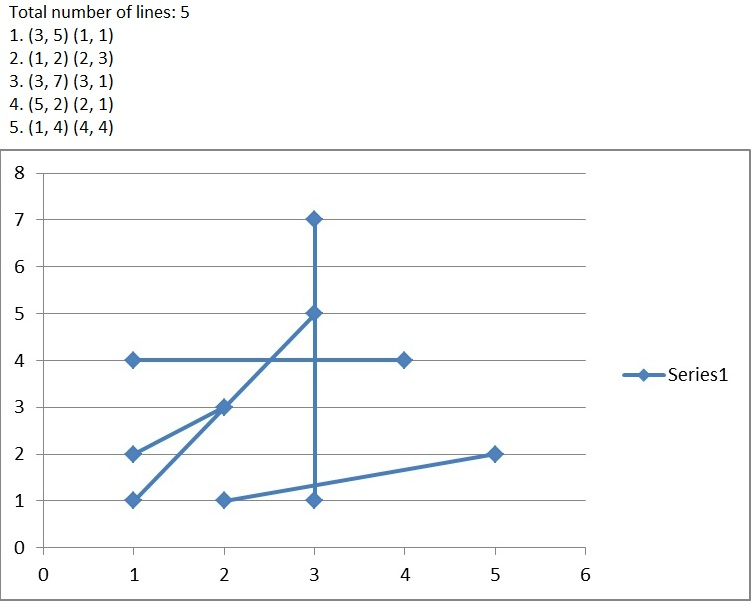
\includegraphics[width=5in, height=3in]{Figures/Figure25}}
  \end{center}
  \centering
	\parbox{5in}{\caption{Graphical representation of program input.} \label{fig25}} 
\end{figure}

The following figures shows the sample output of the program for non-optimized as well as optimized mode of the algorithm. The time taken for the algorithm to run to completion for non-optimized mode is 0.0427698 (Figure.~\ref{fig26}) and the time taken for the algorithm to run to completion for optimized mode is 0.0392279 seconds (Figure.~\ref{fig27}). It can be clearly seen that there is a slight improvement in milliseconds when the program is run in optimzied mode as compared to non-optimized mode. In this particular case there is an improvement of 0.0035419 seconds.
\begin{figure}[ht]
  \begin{center}
   	\fbox{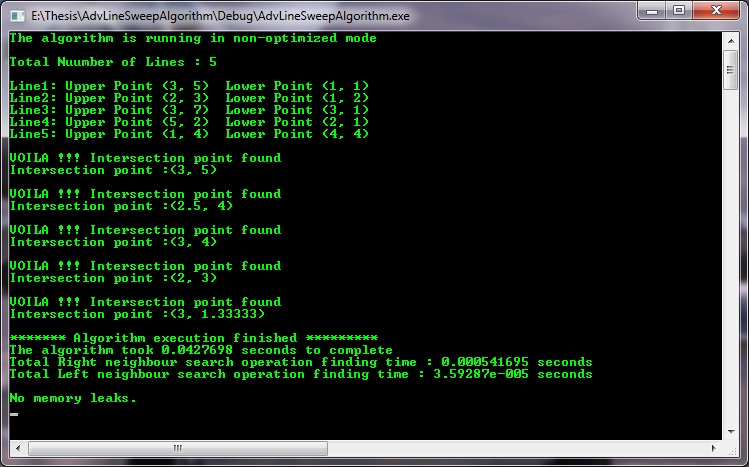
\includegraphics[width=5in, height=3.5in]{Figures/Figure26}}
  \end{center}
  \centering
	\parbox{5in}{\caption{Program output (non-optimized mode).} \label{fig26}} 
\end{figure}
\begin{figure}[ht]
  \begin{center}
   	\fbox{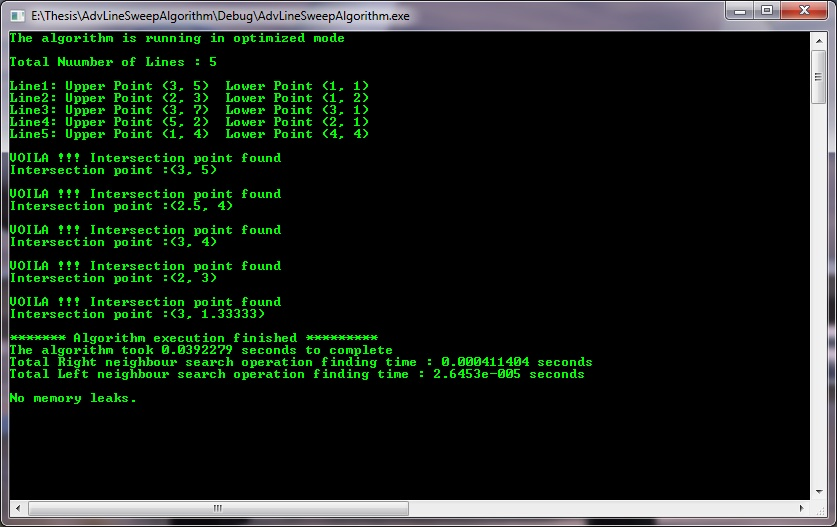
\includegraphics[width=5in, height=3.5in]{Figures/Figure27}}
  \end{center}
  \centering
	\parbox{5in}{\caption{Program output (optimized mode).} \label{fig27}} 
\end{figure}

\clearpage
\section{Results}
Table \ref{tab4} shows the statistical analysis of the neighbor search operation execution time. The program was run on 10 different set of line segments comprising of 5, 50 and 100 set of segments. The line segments were generated using a random number generator program. A generalized random number generator program which is used by the algorithm is provided in Appendix~C.
\begin{table}[hbt]
  \begin{minipage}{6.5in}
	\caption{Statistical Analysis of Neighbor Search Operation on Different Set of Line Segments \label{tab4}}
    \begin{tabular}{||p{1cm}|p{2.5cm}|p{2.5cm}|p{2cm}|p{2cm}|p{2cm}|p{2cm}||}    \hline
       & \multicolumn{2}{|c|}{5 Line Segments} & \multicolumn{2}{|c|}{50 Line Segments} & \multicolumn{2}{|c|}{100 Line Segments} \\ \hline \hline
	   Set & {\it O}(log n) in \newline seconds & {\it O}(1) in \newline seconds & {\it O}(log n) in \newline seconds & {\it O}(1) in \newline seconds & {\it O}(log n) in \newline seconds & {\it O}(1) in \newline seconds \\ \hline
		1 & 0.000585915 & 0.00042009 & 0.0695221 & 0.0584651 & 1.00176 & 0.95164 \\ \hline
		2 & 0.000459967 & 0.000390083 & 0.0536898 & 0.0527888 & 1.19473 & 1.00375 \\ \hline
		3 & 0.000600128 & 0.00055275 & 0.0654452 & 0.0585796 & 1.33972 & 1.11274 \\ \hline
		4 & 0.000571701 & 0.00037508 & 0.0778181 & 0.0547813 & 1.53637 & 1.23689 \\ \hline
		5 & 0.000551170 & 0.000290194 & 0.0508597 & 0.0450012 & 1.64585 & 1.43758 \\ \hline
		6 & 0.000653429 & 0.000301643 & 0.0795048 & 0.0634976 & 1.51176 & 1.38512 \\ \hline
		7 & 0.000414957 & 0.000206491 & 0.0559955 & 0.0466448 & 2.64648 & 2.10963 \\ \hline
		8 & 0.000413378 & 0.000442595 & 0.0591459 & 0.0310854 & 2.10897 & 1.89210 \\ \hline
		9 & 0.000528271 & 0.000338362 & 0.0666241 & 0.0578201 & 1.53587 & 1.31641 \\ \hline
		10 & 0.000595785 & 0.000325333 & 0.0822744 & 0.0631846 & 1.60814 & 1.34926 \\ \hline
    \end{tabular}
  \end{minipage}
\end{table}

\noindent
{\it O}(log n) = Non-optimized (traditional) neighbor search operation time complexity.
\newline \noindent {\it O}(1) = Optimized neighbor search operation time complexity.

\section{Discussion}
Thus it can be clearly seen from Table \ref{tab4} that the optimized mode of the algorithm is definitely better than the non-optimized mode. This difference is short for a small number of input lines but increases gradually as the number of lines increase. For instance we should see a significant improvement in the time complexity of the program, if it is given a huge terra bytes of raster image as an input for solving the map overlay problem (Chapter \ref{chap:intro}) which contains millions of lines. Also it can concluded that the optimized mode of the algorithm increases the neighbor search finding time but it does not contribute much in improving the total running time of the algorithm. This might be because of the way I have coded the algorithm and needs furthur investigation.
